 \begin{multicols}{2}
    \begin{enumerate}
 \item 
\begin{tikzpicture}
            \fill[gray] (0,0) -- (-0.5,1) -- (1,1) -- (1.5,0)-- cycle;
              \fill[gray] (0,0) -- (-0.5,-1) -- (1,-1) -- (1.5,0) -- cycle;
        \end{tikzpicture}        
        \item 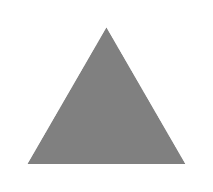
\begin{tikzpicture}
            \fill[gray] (0,0) -- (1,1.73) -- (2,0) -- cycle;
        \end{tikzpicture}
       \item 
\begin{tikzpicture}
            \fill[gray] (0,0) -- (2.2,0) -- (1.85,1.5) -- (0.35,1.5) -- cycle; 
            
        \end{tikzpicture}
        \item  
\begin{tikzpicture}
            \fill[gray] (0,0) rectangle (2,2);
        \end{tikzpicture}
        
        
    \end{enumerate}
    \end{multicols}
